\documentclass[aspectratio=169]{beamer}

% ==== Theme & basic look ====
\usetheme{Madrid}
\usecolortheme{seahorse}
\setbeamertemplate{navigation symbols}{}
\setbeamertemplate{footline}[frame number]

% Font encoding and modern fonts to avoid missing bold-italic shapes
\usepackage[T1]{fontenc}
\usepackage{lmodern}

% Packages for mathematics  
\usepackage{amsmath}  
\usepackage{amsfonts}  
\usepackage{amssymb}  
\usepackage{CJKutf8}
\usepackage{tikz}
\usetikzlibrary{positioning}
% Support for \Tilde macro used throughout
\providecommand{\Tilde}[1]{\tilde{#1}}
\providecommand{\proofname}{Proof}
\newenvironment<>{proofs}[1][\proofname]{%
    \par
    \def\insertproofname{#1.}%
    \usebeamertemplate{proof begin}#2}
  {\usebeamertemplate{proof end}}
\makeatother
\newtheorem{remark}{Remark}

% Math shorthand and vector symbols
\newcommand{\grad}{\nabla}
\newcommand{\EE}{\mathbb{E}}
\newcommand{\dd}{\mathrm{d}}
\newcommand{\kbT}{k_B T}
\newcommand{\vx}{\mathbf{x}}
\newcommand{\R}{\mathbb{R}}
\newcommand{\attn}{\text{Attention}}
\newcommand{\softmax}{\text{softmax}}

% Bold vector/time-indexed variables for autoregressive models
\newcommand{\vxt}{\mathbf{x}_t}
\newcommand{\vxone}{\mathbf{x}_1}
\newcommand{\vxtmone}{\mathbf{x}_{t-1}}
\newcommand{\vxtmoneone}{\mathbf{x}_{t-1:1}}
\newcommand{\vxoneT}{\mathbf{x}_{1:T}}
\newcommand{\vtheta}{\boldsymbol{\theta}}
\newcommand{\vphi}{\boldsymbol{\phi}}
\newcommand{\vz}{\mathbf{z}}
\newcommand{\vc}{\mathbf{c}}

% Title page details:   
\title[Understanding autoregressive models]{Understanding autoregressive models from a mathematical view}  
\author{Pipi Hu}  
\institute[BIMSA]{Beijing Institute of Mathematical Sciences and Applications}  
\date{\today}  

\pgfdeclareimage[width=2cm]{logo}{../figures/logo.png}
\logo{\pgfuseimage{logo}}

% Outline slide (moved to later; avoid frame before \begin{document})

\setbeamertemplate{navigation symbols}{}
\AtBeginSection[]  
{  
    \begin{frame}<beamer>{Outline}         
        \tableofcontents[currentsection]  
    \end{frame}  
}  
  
\AtBeginSubsection[]  
{  
    \begin{frame}<beamer>{Outline}         
        \tableofcontents[currentsection,currentsubsection]  
    \end{frame}  
}  

\begin{document}  
  
% Title slide  
\begin{frame}  
  \titlepage  
\end{frame}  

\begin{frame}{Feynman's words}
\centering
    What I cannot create, I do not understand.
\end{frame}  
  
% Presentation slides  

\section{Preliminary: Autoregressive Models and Sequential Generation}

\begin{frame}{What are autoregressive models?}
Given a sequence $\vxoneT = (x_1, x_2, \ldots, x_T)$, autoregressive models factorize the joint probability as:
\begin{equation}
    p(\vxoneT) = \prod_{t=1}^T p(x_t | \vxtmoneone)
\end{equation}
where $\vxtmoneone = (x_{t-1}, x_{t-2}, \ldots, x_1)$ represents the history.

Key properties:
\begin{itemize}
    \item \textcolor{red}{Sequential generation}: Generate one token at a time
    \item \textcolor{red}{Conditional independence}: Each token depends only on previous tokens
    \item \textcolor{red}{Causal structure}: No future information leakage
\end{itemize}
\end{frame}

\begin{frame}{Mathematical foundation: Chain rule of probability}
The autoregressive factorization follows directly from the chain rule of probability:
\begin{equation}
    p(\vxoneT) = p(x_1) \prod_{t=2}^T p(x_t | \vxtmoneone)
\end{equation}

This factorization is:
\begin{itemize}
    \item \textbf{Always valid}: No assumptions required
    \item \textbf{Exact}: No approximation involved
    \item \textbf{Order-dependent}: Different orderings give different factorizations
\end{itemize}

The challenge is modeling the conditional distributions $p(x_t | \vxtmoneone)$.
\end{frame}

\begin{frame}{Why autoregressive models?}
Advantages of autoregressive modeling:
\begin{enumerate}
    \item \textbf{Simplicity}: Direct application of maximum likelihood
    \item \textbf{Interpretability}: Clear probabilistic interpretation
    \item \textbf{Flexibility}: Can model complex dependencies
    \item \textbf{Training stability}: Well-understood optimization landscape
\end{enumerate}

Challenges:
\begin{enumerate}
    \item \textbf{Sequential generation}: Cannot parallelize during inference
    \item \textbf{Error propagation}: Mistakes compound over time
    \item \textbf{Long-range dependencies}: Hard to capture distant relationships
\end{enumerate}
\end{frame}

\section{Training Autoregressive Models: Maximum Likelihood}

\begin{frame}{Maximum Likelihood Estimation}
Given a dataset $\mathcal{D} = \{\vxoneT^{(i)}\}_{i=1}^N$, we maximize the log-likelihood:
\begin{equation}
    \mathcal{L}(\vtheta) = \sum_{i=1}^N \log p(\vxoneT^{(i)}; \vtheta)
\end{equation}

Substituting the autoregressive factorization:
\begin{equation}
    \mathcal{L}(\vtheta) = \sum_{i=1}^N \sum_{t=1}^T \log p(x_t^{(i)} | \vxtmoneone^{(i)}; \vtheta)
\end{equation}

This decomposes into independent optimization problems for each conditional distribution.
\end{frame}

\begin{frame}{Cross-entropy loss and its interpretation}
For discrete sequences, the loss becomes:
\begin{equation}
    \mathcal{L}(\vtheta) = -\sum_{i=1}^N \sum_{t=1}^T \log p(x_t^{(i)} | \vxtmoneone^{(i)}; \vtheta)
\end{equation}

This is equivalent to minimizing the cross-entropy:
\begin{equation}
    H(p_{\text{data}}, p_{\vtheta}) = \EE_{\vxoneT \sim p_{\text{data}}} \left[ -\sum_{t=1}^T \log p(x_t | \vxtmoneone; \vtheta) \right]
\end{equation}

\textbf{Key insight}: We're learning to predict the next token given the history, which is exactly what we need for generation.
\end{frame}

\begin{frame}{Teacher forcing and training efficiency}
During training, we use \textbf{teacher forcing}:
\begin{itemize}
    \item Input: Ground truth history $\vxtmoneone$
    \item Target: Next token $x_t$
    \item Loss: Cross-entropy between predicted and true distributions
\end{itemize}

This allows:
\begin{enumerate}
    \item \textbf{Parallel training}: All time steps computed simultaneously
    \item \textbf{Stable gradients}: No error propagation during training
    \item \textbf{Efficient optimization}: Standard backpropagation
\end{enumerate}

\textcolor{red}{Note}: Training and inference use different procedures!
\end{frame}

\section{Architectures for Autoregressive Models}

\subsection{RNNs}
\begin{frame}{Recurrent Neural Networks (RNNs)}
The simplest autoregressive architecture:
\begin{equation}
    h_t = f(h_{t-1}, x_{t-1}; \vtheta)
\end{equation}
\begin{equation}
    p(x_t | \vxtmoneone) = g(h_t; \vtheta)
\end{equation}

where $h_t$ is the hidden state and $f, g$ are neural networks.

\textbf{Advantages}:
\begin{itemize}
    \item Natural sequential processing
    \item Parameter sharing across time
    \item Variable-length sequences
\end{itemize}

\textbf{Limitations}:
\begin{itemize}
    \item Vanishing/exploding gradients
    \item Limited long-range dependencies
    \item Sequential computation
\end{itemize}
\end{frame}

\subsection{LSTMs}
\begin{frame}{Long Short-Term Memory (LSTM)}
LSTM addresses RNN limitations with gating mechanisms:
\begin{align}
    f_t &= \sigma(W_f \cdot [h_{t-1}, x_t] + b_f) \quad \text{(forget gate)} \\
    i_t &= \sigma(W_i \cdot [h_{t-1}, x_t] + b_i) \quad \text{(input gate)} \\
    \tilde{C}_t &= \tanh(W_C \cdot [h_{t-1}, x_t] + b_C) \quad \text{(candidate values)} \\
    C_t &= f_t * C_{t-1} + i_t * \tilde{C}_t \quad \text{(cell state)} \\
    o_t &= \sigma(W_o \cdot [h_{t-1}, x_t] + b_o) \quad \text{(output gate)} \\
    h_t &= o_t * \tanh(C_t) \quad \text{(hidden state)}
\end{align}

\textbf{Key innovations}:
\begin{itemize}
    \item \textcolor{red}{Gating}: Control information flow
    \item \textcolor{red}{Cell state}: Long-term memory storage
    \item \textcolor{red}{Gradient flow}: Better backpropagation
\end{itemize}
\end{frame}

\subsection{Transformers}

\begin{frame}{Transformers}
\begin{figure}
    \centering
    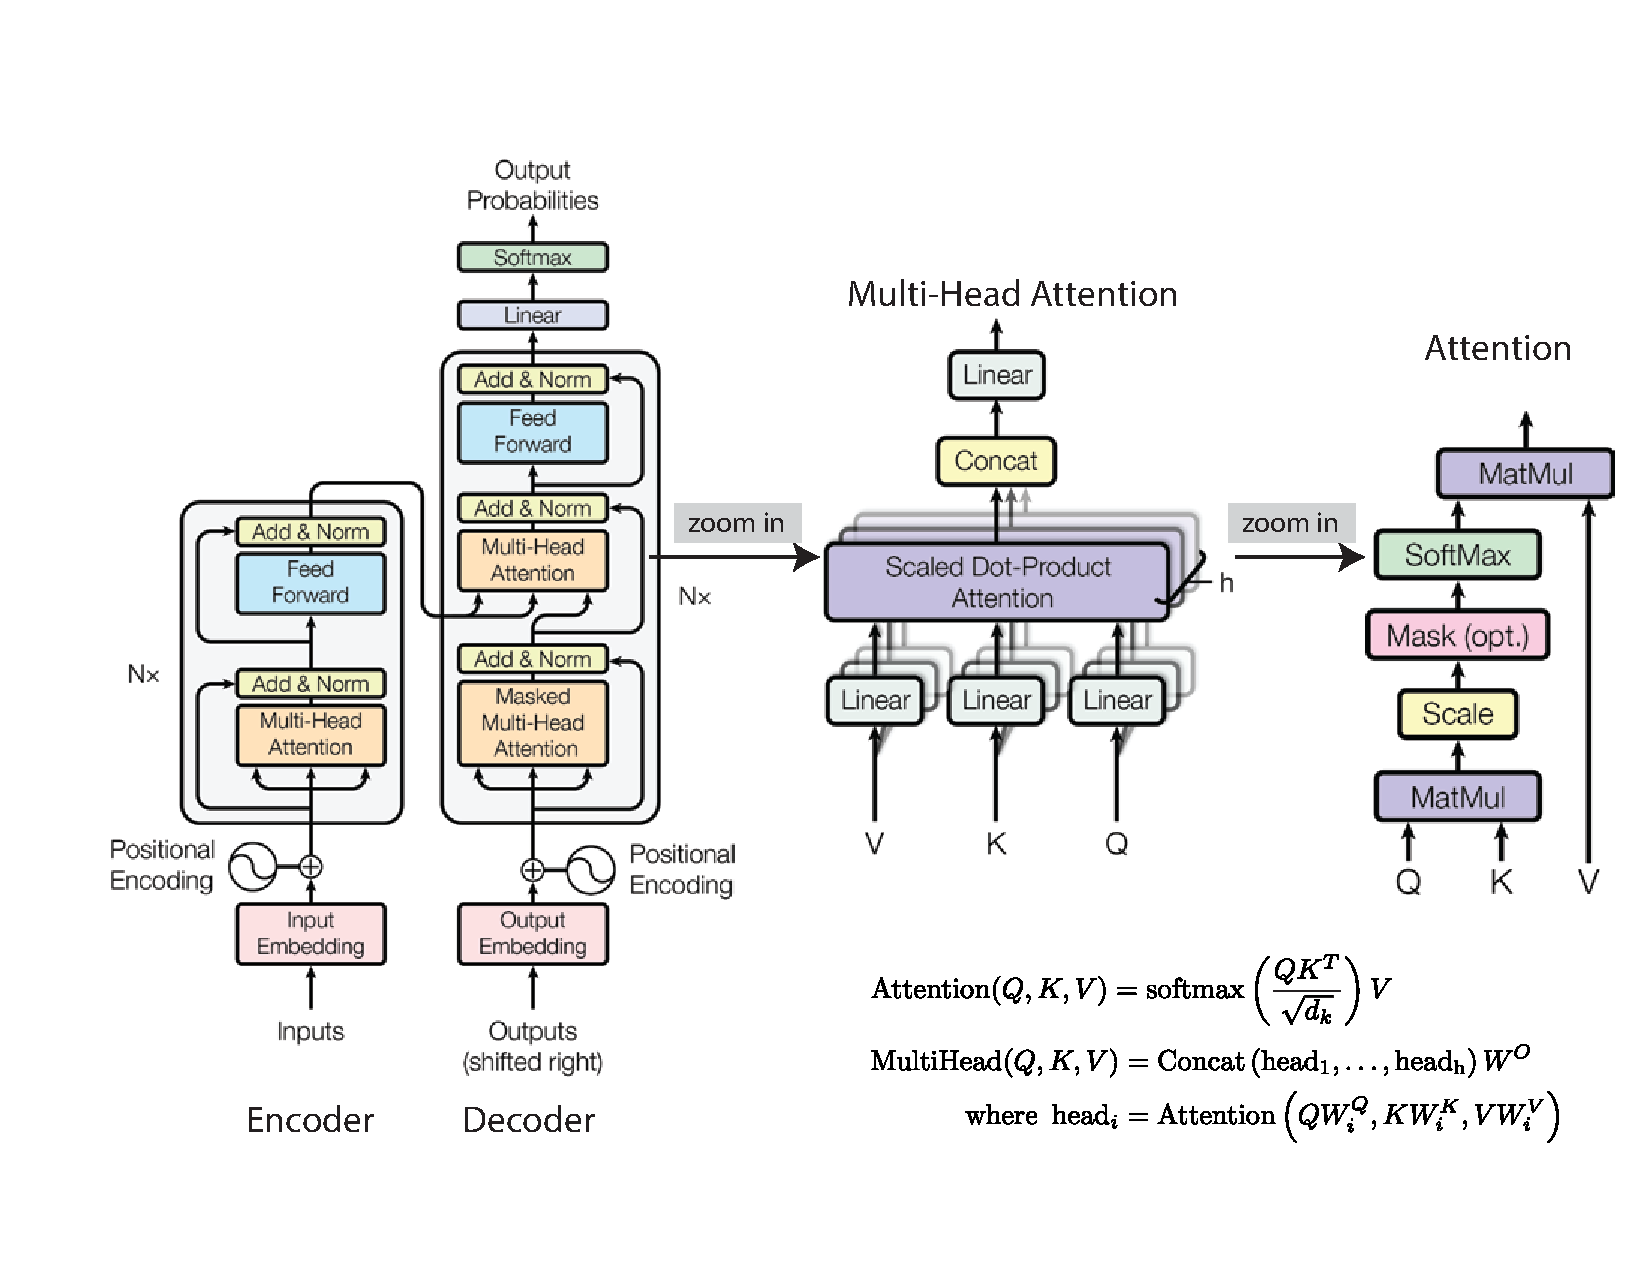
\includegraphics[width=0.75\textwidth]{../figures/transformer.pdf}
\end{figure}
\end{frame}

\begin{frame}{Scaled Dot-Product Attention: Key formula}
  Inputs: queries $Q\in\R^{n\times d_k}$, keys $K\in\R^{n\times d_k}$, values $V\in\R^{n\times d_v}$.
  \begin{align}
  \attn(Q,K,V) &= \softmax\!\left(\frac{QK^\top}{\sqrt{d_k}} + M\right) V, \label{eq:attn}
  \end{align}
  where $M$ is an optional mask (e.g., $M_{ij}=-\infty$ for $j>i$ in autoregressive decoding).
  \begin{itemize}
  \item Scaling by $\sqrt{d_k}$ keeps gradients in a reasonable range.
  \item \textbf{Interpretation}: each token re-weights all values using similarity to keys.
  \end{itemize}
  \end{frame}
  
  \begin{frame}{Multi-Head Attention (MHA)}
  \begin{align}
  \mathrm{MHA}(X) &= \mathrm{Concat}(H_1,\dots,H_h) \, W^O,\\
  H_i &= \attn(X W_i^Q,\, X W_i^K,\, X W_i^V),\quad i=1,\dots,h.
  \end{align}
  \begin{itemize}
  \item Heads attend to different subspaces/patterns.
  \item Residual + LayerNorm around MHA and FFN blocks stabilize training.
  \end{itemize}
  \end{frame}


\begin{frame}{Understanding the Transformer architecture from a mathematical view}
\begin{itemize}
    \item Input embedding: $X \in \R^{n\times d}$;
    \item Query, key, value projections: $Q = X W_Q$, $K = X W_K$, $V = X W_V$; (Notatiion slightly different from the original paper)
    \item Attention: $A = \softmax(QK^\top / \sqrt{d_k}) + M$;
    \item Output: $O = AV$;
\end{itemize}

\vspace{-0.5em}
\begin{center}
\begin{tikzpicture}[scale=0.7, every node/.style={scale=0.7}, node distance=0.21cm]
    % Input X
    \node[draw, rectangle, minimum width=1.5cm, minimum height=2cm, fill=blue!20] (X) at (0,0) {$X$};
    \node[below=of X] {$n \times d$};
    
    % Projections
    \node[draw, rectangle, minimum width=1cm, minimum height=1.5cm, fill=green!20] (WQ) at (2.5,0.5) {$W_Q$};
    \node[below=of WQ] {$d \times d_k$};
    \node[draw, rectangle, minimum width=1cm, minimum height=1.5cm, fill=green!20] (WK) at (2.5,-0.5) {$W_K$};
    \node[below=of WK] {$d \times d_k$};
    \node[draw, rectangle, minimum width=1cm, minimum height=1.5cm, fill=green!20] (WV) at (2.5,-1.5) {$W_V$};
    \node[below=of WV] {$d \times d_v$};
    
    % Q, K, V
    \node[draw, rectangle, minimum width=1.5cm, minimum height=1.5cm, fill=orange!20] (Q) at (5,0.5) {$Q$};
    \node[below=of Q] {$n \times d_k$};
    \node[draw, rectangle, minimum width=1.5cm, minimum height=1.5cm, fill=orange!20] (K) at (5,-0.5) {$K$};
    \node[below=of K] {$n \times d_k$};
    \node[draw, rectangle, minimum width=1.5cm, minimum height=1.5cm, fill=orange!20] (V) at (5,-1.5) {$V$};
    \node[below=of V] {$n \times d_v$};
    
    % QK^T
    \node[draw, rectangle, minimum width=1.5cm, minimum height=1.5cm, fill=yellow!20] (QKT) at (7.5,0) {$QK^\top$};
    \node[below=of QKT] {$n \times n$};
    \node[above=of QKT, node distance=0.4cm] {$\div \sqrt{d_k}$};
    
    % Attention matrix A
    \node[draw, rectangle, minimum width=1.5cm, minimum height=1.5cm, fill=red!20] (A) at (10,0) {$A$};
    \node[below=of A] {$n \times n$};
    
    % Output O
    \node[draw, rectangle, minimum width=1.5cm, minimum height=2cm, fill=purple!20] (O) at (12.5,0) {$O$};
    \node[below=of O] {$n \times d_v$};
    
    % Arrows
    \draw[->, thick] (X) -- (WQ);
    \draw[->, thick] (X) -- (WK);
    \draw[->, thick] (X) -- (WV);
    \draw[->, thick] (WQ) -- (Q);
    \draw[->, thick] (WK) -- (K);
    \draw[->, thick] (WV) -- (V);
    \draw[->, thick] (Q) -- (QKT);
    \draw[->, thick] (K) -- (QKT) node[midway, above, sloped, font=\scriptsize] {$\top$};
    \draw[->, thick] (QKT) -- (A) node[midway, above, font=\scriptsize] {$\softmax$};
    \draw[->, thick] (A) -- (O);
    \draw[->, thick] (V) -- (O);
\end{tikzpicture}
\end{center}
\begin{remark}
    Understand the Transformer architecture by block matrix, e.g., $(AB)_k = \sum_{k}A_{ki}B_i$.
\end{remark}
\end{frame}

\section{Rotational Positional Encoding (RoPE)}
\begin{frame}{Motivation: Positional Information in Transformers}
  \begin{itemize}
    \item Vanilla self-attention is permutation invariant:
    \[
      \text{Attn}(X) = \text{softmax}\!\left(\frac{QK^\top}{\sqrt{d}}\right)V
    \]
    \item We need positional information to distinguish sequences like
          ``A B C'' vs.\ ``C B A''.
    \item Classical approaches:
    \begin{itemize}
      \item \emph{Absolute} positional encodings (e.g.\ sinusoidal or learned vectors added to token embeddings).
      \item \emph{Relative} positional encodings (e.g.\ bias as a function of $n-m$ added to attention logits).
    \end{itemize}
    \item Absolute encodings tie the model to a fixed maximum length and do not naturally express relative positions.
  \end{itemize}
\end{frame}

%------------------------------------------------
\begin{frame}{Idea of RoPE}
  \begin{itemize}
    \item RoPE: encode position by applying a \textbf{rotation} to queries and keys in each attention head.
    \item For a token at position $m$, instead of
      \[
        q_m = W_Q x_m,\quad k_m = W_K x_m,
      \]
      RoPE uses
      \[
        \tilde{q}_m = R_m q_m,\quad \tilde{k}_m = R_m k_m,
      \]
      where $R_m$ is a block-diagonal rotation matrix depending on position $m$.
    \item Crucial property:
      \[
        \langle \tilde{q}_m,\tilde{k}_n\rangle
        = \langle q_m, R_{n-m} k_n\rangle,
      \]
      so the attention score depends on the \textbf{relative position} $n-m$.
  \end{itemize}
\end{frame}

%------------------------------------------------
\begin{frame}{Rotations in 2D Subspaces}
  \begin{itemize}
    \item Let head dimension be $d_h$, and group coordinates into 2D blocks:
      \[
        q_m = \big( q_m^{(1)}, q_m^{(2)}, \dots, q_m^{(d_h/2)} \big),
      \]
      where each $q_m^{(j)} \in \mathbb{R}^2$.
    \item For each block $j$ we pick a frequency $\omega_j > 0$ and define a 2D rotation:
      \[
        R_m^{(j)} =
        \begin{bmatrix}
          \cos(\omega_j m) & -\sin(\omega_j m)\\
          \sin(\omega_j m) & \phantom{-}\cos(\omega_j m)
        \end{bmatrix}.
      \]
    \item The full rotation $R_m$ is block diagonal:
      \[
        R_m = \mathrm{diag}\big(R_m^{(1)}, R_m^{(2)}, \dots, R_m^{(d_h/2)}\big).
      \]
    \item Apply $R_m$ to $q_m$ and $k_m$ to get position-aware vectors $\tilde{q}_m, \tilde{k}_m$.
  \end{itemize}
\end{frame}

%------------------------------------------------
\begin{frame}{Complex-Valued View and Relative Positions}
  \begin{itemize}
    \item A 2D vector $q_m^{(j)} = (a,b)$ can be seen as a complex number $z = a + i b$.
    \item The rotation $R_m^{(j)}$ corresponds to multiplying by $e^{i\omega_j m}$:
      \[
        \tilde{z}_m^{(j)} = e^{i\omega_j m} z_m^{(j)}.
      \]
    \item For positions $m$ and $n$:
      \[
        \tilde{z}_m^{(j)} \,\overline{\tilde{z}_n^{(j)}}
        = e^{i\omega_j (m-n)} z_m^{(j)} \overline{z_n^{(j)}},
      \]
      so the phase difference depends only on $(m-n)$.
    \item Summing over all blocks yields
      \[
        \langle \tilde{q}_m,\tilde{k}_n\rangle
        = \langle q_m, R_{n-m} k_n\rangle
        = f(q_m,k_n,n-m),
      \]
      an attention score that is \textbf{equivariant to shifts} and carries relative positional information.
  \end{itemize}
\end{frame}

%------------------------------------------------
\begin{frame}{Multi-Head Attention with RoPE}
  \begin{itemize}
    \item For each head $h$:
      \[
        q_m^{(h)} = W_Q^{(h)} x_m,\quad
        k_m^{(h)} = W_K^{(h)} x_m.
      \]
    \item Apply RoPE:
      \[
        \tilde{q}_m^{(h)} = R_m^{(h)} q_m^{(h)},\quad
        \tilde{k}_m^{(h)} = R_m^{(h)} k_m^{(h)}.
      \]
    \item Attention logits for head $h$:
      \[
        s_{m,n}^{(h)} =
        \frac{1}{\sqrt{d_h}}
        \big\langle \tilde{q}_m^{(h)}, \tilde{k}_n^{(h)}\big\rangle.
      \]
    \item Frequencies $\{\omega_j\}$ are typically shared across heads and chosen as a geometric progression, analogous to sinusoidal positional encodings.
  \end{itemize}
\end{frame}

%------------------------------------------------
\begin{frame}{Frequency Schedule and Length Extrapolation}
  \begin{itemize}
    \item Frequencies are usually defined as
      \[
        \omega_j = \theta^{-2j/d_h},\quad
        \theta > 1,
      \]
      where $j = 0,1,\dots,d_h/2-1$.
    \item Low frequencies capture long-range structure, high frequencies capture fine-grained local patterns.
    \item Because RoPE is defined analytically for any integer position $m$, it can be \emph{extrapolated} to longer sequences than seen during training (though with practical limits).
    \item Variants such as ``scaled RoPE'' or ``XPOS'' modify the effective frequency or add per-dimension scaling to improve length extrapolation and numerical stability.
  \end{itemize}
\end{frame}

\section{Sampling and Generation Strategies}

\begin{frame}{Greedy decoding}
The simplest generation strategy:
\begin{equation}
    x_t = \arg\max_{x} p(x | \vxtmoneone; \vtheta)
\end{equation}

\textbf{Properties}:
\begin{itemize}
    \item Deterministic: Same input always produces same output
    \item Fast: Single forward pass per token
    \item Often suboptimal: Local decisions may not be globally optimal
\end{itemize}

\textbf{Issues}:
\begin{itemize}
    \item \textcolor{red}{Repetition}: May get stuck in loops
    \item \textcolor{red}{Lack of diversity}: Always chooses most likely token
    \item \textcolor{red}{Mode collapse}: May not explore the full distribution
\end{itemize}
\end{frame}

\begin{frame}{Random sampling}
Sample from the full distribution:
\begin{equation}
    x_t \sim p(x | \vxtmoneone; \vtheta)
\end{equation}

\textbf{Advantages}:
\begin{itemize}
    \item \textcolor{red}{Diversity}: Explores the full distribution
    \item \textcolor{red}{Natural}: Reflects model uncertainty
    \item \textcolor{red}{Flexibility}: Can control randomness
\end{itemize}

\textbf{Challenges}:
\begin{itemize}
    \item \textcolor{red}{Quality control}: May generate low-quality sequences
    \item \textcolor{red}{Consistency}: Less predictable output
    \item \textcolor{red}{Evaluation}: Harder to assess quality
\end{itemize}
\end{frame}

\begin{frame}{Temperature scaling and nucleus sampling}
\textbf{Temperature scaling}:
\begin{equation}
    p_{\text{temp}}(x | \vxtmoneone) = \frac{\exp(f(x, \vxtmoneone) / \tau)}{\sum_{x'} \exp(f(x', \vxtmoneone) / \tau)}
\end{equation}

where $x$ is a token candidate from the vocabulary $\mathcal{V}$ for $x_t$,
 $f(x, x_{t-1:1})$ is the logit (pre-softmax output) for $x$ given the history $x_{t-1:1}$, and $\tau > 0$ controls randomness:
\begin{itemize}
    \item $\tau \to 0$: Greedy decoding
    \item $\tau = 1$: Original distribution
    \item $\tau > 1$: More random
\end{itemize}

\textbf{Nucleus sampling, i.e., top-$p$ sampling} (Holtzman et al., 2019):
\begin{equation}
    \text{Select smallest } V \text{ such that } \sum_{x \in V} p(x | \vxtmoneone) \geq p
\end{equation}
Then sample from the truncated distribution.
\end{frame}

\begin{frame}{Limiting behavior of temperature scaling I}
Consider logits $f(x,\vxtmoneone)$ over a finite dictionary $\mathcal{V}$ and the temperature-scaled distribution
\[
  p_\tau(x) = \frac{\exp(f(x,\vxtmoneone)/\tau)}{\sum_{x' \in \mathcal{V}} \exp(f(x',\vxtmoneone)/\tau)}.
\]
\textbf{Claim 1 (greedy limit).} Let $x^\star = \arg\max_{x} f(x,\vxtmoneone)$ and assume it is unique. Then
\[
  \lim_{\tau\to 0^+} p_\tau(x) = \delta_{x^\star}(x).
\]
\textbf{Proof.} For any $x\neq x^\star$, we have $f(x,\vxtmoneone) - f(x^\star,\vxtmoneone) < 0$, hence
\[
  \frac{p_\tau(x)}{p_\tau(x^\star)}
  = \exp\Big(\tfrac{f(x,\vxtmoneone)-f(x^\star,\vxtmoneone)}{\tau}\Big) \xrightarrow[\tau\to 0^+]{} 0,
\]
so all mass concentrates on $x^\star$. (We can also divided by $exp(f(x^\star,\vxtmoneone)/\tau)$ on $p_\tau(x)$ and $p_\tau(x^\star)$ to get the same result with $p_\tau(x^\star) = 1$ and $p_\tau(x) = 0$ for $x \neq x^\star$.)
\end{frame}

\begin{frame}{Limiting behavior of temperature scaling II}
We keep the same definition
\[
  p_\tau(x) = \frac{\exp(f(x,\vxtmoneone)/\tau)}{\sum_{x' \in \mathcal{V}} \exp(f(x',\vxtmoneone)/\tau)}.
\]
\textbf{Claim 2 (uniform limit).} As $\tau\to\infty$,
\[
  p_\tau(x) \;\longrightarrow\; \frac{1}{|\mathcal{V}|}\quad \text{for all }x\in\mathcal{V}.
\]
\textbf{Proof.} Using $\exp(f/\tau) = 1 + \mathcal{O}(1/\tau)$ as $\tau\to\infty$, we have
\[
  p_\tau(x) = \frac{1 + \mathcal{O}(1/\tau)}{|\mathcal{V}| + \mathcal{O}(1/\tau)}
  \xrightarrow[\tau\to\infty]{} \frac{1}{|\mathcal{V}|}.
\]
\end{frame}



\section{Evaluation and Challenges}

\begin{frame}{Evaluation metrics for autoregressive models}
\textbf{Perplexity}:
\begin{equation}
    \text{Perplexity} = \exp\left(-\frac{1}{T} \sum_{t=1}^T \log p(x_t | \vxtmoneone; \vtheta)\right)
\end{equation}

\textbf{Other metrics}:
\begin{itemize}
    \item \textcolor{red}{BLEU}: N-gram overlap with reference
    \item \textcolor{red}{ROUGE}: Recall-oriented evaluation
    \item \textcolor{red}{BERTScore}: Semantic similarity using BERT
    \item \textcolor{red}{Human evaluation}: Subjective quality assessment
\end{itemize}

\textbf{Challenges}:
\begin{itemize}
    \item \textcolor{red}{No single metric}: Different tasks need different metrics
    \item \textcolor{red}{Reference dependence}: Many metrics need reference text
    \item \textcolor{red}{Human evaluation}: Expensive and subjective
\end{itemize}
\end{frame}

\begin{frame}{Information-theoretic perspective}
The entropy of an autoregressive model is:
\begin{equation}
    H(p_{\vtheta}) = \EE_{\vxoneT \sim p_{\vtheta}} \left[ -\sum_{t=1}^T \log p(x_t | \vxtmoneone; \vtheta) \right]
\end{equation}

\textbf{Key insights}:
\begin{itemize}
    \item \textcolor{red}{Conditional entropy}: $H(X_t | X_{t-1:1}) \leq H(X_t)$
    \item \textcolor{red}{Chain rule}: $H(X_{1:T}) = \sum_{t=1}^T H(X_t | X_{t-1:1})$
    \item \textcolor{red}{Compression}: Autoregressive models compress information
\end{itemize}

\textbf{Compression ratio}:
\begin{equation}
    \text{Compression} = \frac{H(X_{1:T})}{T \log V} = \frac{\sum_{t=1}^T H(X_t | X_{t-1:1})}{T \log V}
\end{equation}

Lower compression ratio means better modeling of dependencies.
\end{frame}

\begin{frame}{Large language models and scaling laws}
\textbf{Scaling laws} (Kaplan et al., 2020):
\begin{equation}
    L(N, D) = \left(\frac{N_c}{N}\right)^{\alpha_N} + \left(\frac{D_c}{D}\right)^{\alpha_D}
\end{equation}

where $N$ is model size, $D$ is dataset size, and $L$ is loss.

\textbf{Key findings}:
\begin{itemize}
    \item \textcolor{red}{Power law scaling}: Performance improves predictably with scale
    \item \textcolor{red}{Emergent abilities}: New capabilities emerge at certain scales
    \item \textcolor{red}{Efficient scaling}: Larger models are more sample-efficient
\end{itemize}

\textbf{Implications}:
\begin{itemize}
    \item \textcolor{red}{Compute requirements}: Training costs scale dramatically
    \item \textcolor{red}{Data requirements}: Need massive datasets
    \item \textcolor{red}{Architecture choices}: Transformer scales well
\end{itemize}
\end{frame}

\begin{frame}{Common challenges and limitations}
\textbf{Training challenges}:
\begin{enumerate}
    \item \textcolor{red}{Exposure bias}: Training uses ground truth, inference uses model predictions
    \item \textcolor{red}{Teacher forcing mismatch}: Different distributions during training and inference
    \item \textcolor{red}{Long sequences}: Gradient vanishing/exploding
\end{enumerate}

\textbf{Generation challenges}:
\begin{enumerate}
    \item \textcolor{red}{Repetition}: Models may repeat phrases or sentences
    \item \textcolor{red}{Coherence}: Long-range dependencies hard to maintain
    \item \textcolor{red}{Diversity vs. Quality}: Trade-off between exploration and exploitation
\end{enumerate}

\textbf{Computational challenges}:
\begin{enumerate}
    \item \textcolor{red}{Sequential generation}: Cannot parallelize inference
    \item \textcolor{red}{Memory requirements}: Need to store full history
    \item \textcolor{red}{Scalability}: Training large models is expensive
\end{enumerate}
\end{frame}

\section{Open Questions and Research Directions}

\begin{frame}{Open questions}
If you are interested in these questions, please feel free to write an email to me {\color{red}(\href{mailto:hpp@bimsa.cn}{hpp@bimsa.cn})} with your comments.

\begin{enumerate}[(1.)]
    \item How can we design better non-autoregressive models that maintain quality while enabling parallel generation?
    \item Could we use auto-regressive models to model the joint distribution of images and text naturally?
    \item How do we balance the trade-off between generation speed and quality in practical applications?
    \item What role do autoregressive models play in the broader landscape of generative AI, and how do they compare to diffusion models and other approaches?
    \item Can we develop theoretical frameworks to understand when autoregressive models will succeed or fail?
\end{enumerate}
\end{frame}


% Thank you slide  
\begin{frame}{Welcome inputs}  
  \centering  
  Any comments?
  \\[2em]
  Welcome your inputs!  
\end{frame}  
  
\end{document}
